\documentclass{standalone}
\usepackage{tikz}
\usepackage{ctex,siunitx,ninecolors}
\setCJKmainfont{Noto Serif CJK SC}
\usepackage{tkz-euclide}
\usepackage{amsmath}
\usetikzlibrary{patterns, calc}
\usetikzlibrary {decorations.pathmorphing, decorations.pathreplacing, decorations.shapes}
\begin{document}
\small
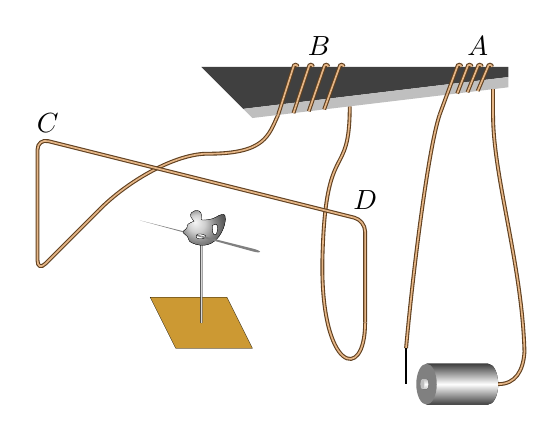
\begin{tikzpicture}[scale=1.3]
  \begin{scope}[xscale=-0.5,yscale=0.5]
  \draw[fill=brown!80!yellow,ultra thin](-1,-0.5)--(0.5,-0.5)--(1,0.5)--(-0.5,0.5)--cycle;
  \fill[left color=gray,right color=gray,middle color=white](-0.02,0)arc(180:360:0.02 and 0.01)--(0.02,1.6)--(-0.02,1.6)--cycle;
  \fill[gray](1.2,2)--(0,1.7)--(0,1.67)--cycle;
  \fill[ball color=lightgray,draw=black,ultra thin]( 0.145,1.985)..controls( 0.373,1.885)and( 0.222,1.897)..
  ( 0.299,1.833)..controls( 0.330,1.812)and( 0.405,1.773)..
  ( 0.316,1.724)..controls( 0.222,1.667)and( 0.275,1.600)..
  ( 0.194,1.565)..controls(-0.315,1.329)and(-0.519,1.952)..
  (-0.461,2.097)..controls(-0.445,2.142)and(-0.343,2.101)..
  (-0.289,2.064)..controls(-0.198,2.011)and(-0.094,2.008)..
  (-0.046,2.007)..controls(-0.035,2.009)and(-0.005,1.999)..
  ( 0.003,2.020)..controls( 0.012,2.049)and( 0.000,2.050)..
  (-0.001,2.104)..controls(-0.002,2.249)and( 0.252,2.203)..
  ( 0.204,2.067)..controls( 0.179,2.011)and( 0.174,2.031)..cycle
  (-0.214,1.901)..controls(-0.369,1.987)and(-0.316,1.814)..
  (-0.297,1.732)..controls(-0.205,1.671)and(-0.216,1.829)..cycle
  ( 0.101,1.681)..controls( 0.121,1.794)and(-0.209,1.704)..
  (-0.044,1.646)..controls( 0.007,1.631)and( 0.097,1.635)..cycle;
  \fill[gray](0,1.7)--(-1,1.45)..controls(-1.2,1.4)and(-1.2,1.34)..(-1,1.395)--(0,1.67);
  \end{scope}
\begin{scope}[xshift=0.2cm]
  \fill[top color=darkgray,bottom color=darkgray,middle color=white](2.0,-0.8)--(2.6,-0.8)arc(-90:90:0.1 and 0.2)--(2.0,-0.4)--cycle;
  \fill[gray](2.0,-0.6)ellipse(0.1 and 0.2);
  \fill[top color=lightgray,bottom color=lightgray,middle color=white](1.96,-0.65)--(2.0,-0.65)arc(-90:90:0.02 and 0.05)--(1.96,-0.55)--cycle;
  \fill[lightgray](1.96,-0.6)ellipse(0.02 and 0.05);
\end{scope}
\draw[double=brown8,brown!50!black](-1.000,1.100)..controls(-0.718,1.388)and(-0.239,1.660)..
( 0.076,1.651)..controls( 0.624,1.653)and( 0.657,1.830)..( 0.750,2.030)
(1.450, 2.114)..controls(1.450, 1.362)and(1.211, 1.830)..
(1.183, 0.621)..controls(1.161,-0.480)and(1.600,-0.591)..(1.600, 0.000)
(2.328, 2.031)..controls(2.223, 1.722)and(2.076, 0.586)..(2.0,-0.25)
(2.850, 2.031)..controls(2.850, 1.430)and(3.134, 0.566)..
(3.157,-0.284)..controls(3.145,-0.468)and(3.072,-0.600)..(2.900,-0.600);
\draw[rounded corners,double=brown8,brown!50!black](-1.0,1.1)--(-1.6,0.5)--(-1.6,1.8)--(1.6,1)--(1.6,0);
\fill[darkgray](0,2.5)--(0.4107,2.0893)--(3,2.4)--(3,2.5);
\fill[lightgray](0.4107,2.0893)--(0.5,2.0)--(3,2.3)--(3,2.4);
\draw[double=brown8,brown!50!black](0.75,2.03)--(0.9,2.5)arc(180:0:0.02);
\draw[double=brown8,brown!50!black](0.9,2.048)--(1.05,2.5)arc(180:0:0.02);
\draw[double=brown8,brown!50!black](1.05,2.066)--(1.2,2.5)arc(180:0:0.02);
\draw[double=brown8,brown!50!black](1.2,2.084)--(1.35,2.5)arc(180:0:0.02);
\draw[double=brown8,brown!50!black](2.3277,2.0314)--(2.5,2.5)arc(180:0:0.02);
\draw[double=brown8,brown!50!black](2.5,2.24)--(2.6,2.5)arc(180:0:0.02);
\draw[double=brown8,brown!50!black](2.6,2.252)--(2.7,2.5)arc(180:0:0.02);
\draw[double=brown8,brown!50!black](2.7,2.264)--(2.8,2.5)arc(180:0:0.02);
\draw[double=brown8,brown!50!black](2.85,2.282)--(2.85,2.0314);
\draw(2.0,-0.25)--(2.0,-0.6);
\node at (2.7,2.7) {$A$};
\node at (1.15,2.7) {$B$};
\node at (-1.5,1.95) {$C$};
\node at (1.6,1.2) {$D$};
\end{tikzpicture}
\end{document}